\documentclass[preview]{standalone}
% \documentclass{scrartcl}
\usepackage{tikz}
\begin{document}
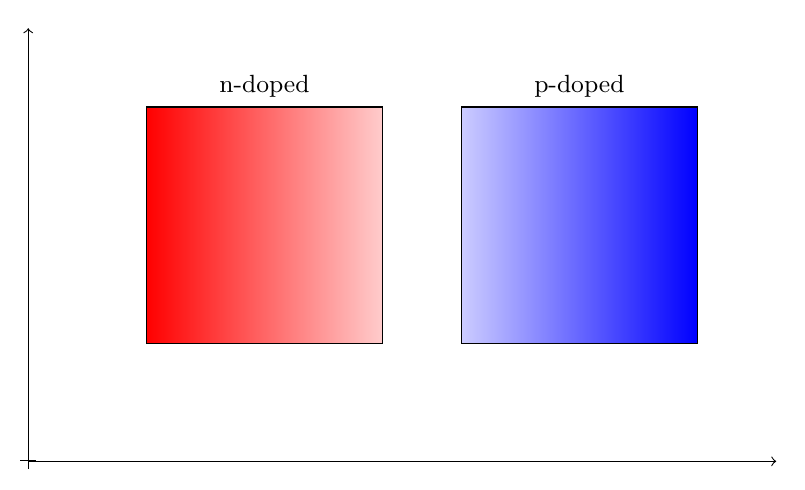
\begin{tikzpicture}

\coordinate(lowerleft) at (0,0);
\coordinate(upperright) at (10,5);

\draw[|->] (lowerleft) ++ (-0.5,-0.5) to ++ (0,5.5);
\draw[|->] (lowerleft) ++ (-0.5,-0.5) to ++ (9.5,0);

\coordinate(Aa) at (1, 1);
\coordinate(Ab) at (1, 4);
\coordinate(Ac) at (4, 4);
\coordinate(Ad) at (4, 1);

\coordinate(Ba) at (5, 1);
\coordinate(Bb) at (5, 4);
\coordinate(Bc) at (8, 4);
\coordinate(Bd) at (8, 1);

\path[left color=red, right color=red!20]
  (Aa) rectangle (Ac);
\path[left color=blue!20, right color=blue]
  (Ba) rectangle (Bc);

\draw (Aa)
  to (Ab)
  to node[above]{\small n-doped} (Ac)
  to (Ad)
  to (Aa);

\draw (Ab) ++ (0,1);

\draw (Ba)
  to (Bb)
  to node[above]{\small p-doped} (Bc)
  to (Bd)
  to (Ba);


\end{tikzpicture}

\end{document}
